\chapter{Introduction}\label{CH:introduction}
Above Earth's atmosphere are the Van Allen radiation belts, a complex and dynamic plasma environment that can effect our technology-driven society. These effects include: a higher radiation dose for astronauts and cosmonauts, higher chance of spacecraft failure due to single event upsets that can lead to catastrophic latchups, cumulative degradation of silicon (changing the silicon doping) from an extended radiation dose that can degrade a transition to the point where it no longer function as a switch, and the degradation of the ozone layer due to the chemical production of NOX and HOX. With these effects in mind, it is no surprise that the radiation belts have been extensively studied since their discovery in the 1960s.

A topic of interest in the space physics community is wave-particle intersections that as we will see later in the introduction, can accelerate particles and scatter them into the atmosphere.

The goal of this dissertation is to study the wave-particle mechanism that scatters microbursts into Earth's atmosphere. This goal will be achieved by first introducing single charged particle motion in electric and magnetic fields, the major particle populations and how they couple in the magnetosphere, and then describe the history and current state of the fields relating to microbursts and wave-particle scattering

\section{Charged Particle Motion in Electric and Magnetic Fields}\label{Intro:particle_motion}
A charged particle trapped in the magnetosphere will experience three types of periodic motion in Earth's nearly dipolar field. The three motions are ultimately due to the Lorentz force that a particle of momentum $\vec{p}$, charge $q$, and velocity $\vec{v}$ experiences in an electric field $\vec{E}$ and magnetic field $\vec{B}$ and is given by
\begin{equation} \label{Intro:Lorentz}
\frac{d\vec{p}}{dt} = q(\vec{E} + \vec{v} \times \vec{B}).
\end{equation} In the magnetosphere, the three periodic motions in decreasing frequency are gyration, bounce, and drift and are schematically shown in Fig. \ref{Intro:motion_diagram}. Each of periodic these motions have a corresponding conserved quantity i.e. an adiabatic invariant. 

\begin{figure}
\includegraphics[width=\textwidth]{1_three_motions.png}
\caption{A diagram of the three motions that a charged particle experiences in Earth's dipole magnetic field. These motions are: gyration about the magnetic field line, bounce motion between the magnetic poles, and azimuthal drift around the Earth. Figure from \citep{Baumjohann1997}.}
\label{Intro:motion_diagram}
\end{figure}


The highest frequency periodic motion is on the order of a kHz in the magnetosphere and is gyration about a magnetic field of magnitude $B$. This motion is circular with a Larmor radius of 
\begin{equation}
r = \frac{m v_\perp}{|q| B}
\end{equation} where $m$ is the mass and $v_\perp$ the particle velocity perpendicular to $\vec{B}$. This motion has a corresponding gyrofrequency 
\begin{equation}
\Omega = \frac{|q| B}{m}
\end{equation} in units of radians/second. The corresponding adiabatic invariant can be found by integrating the particle's canonical momentum around the particle's path
\begin{equation}
J_i = \oint (\vec{p} + q \vec{A}) \cdot d\vec{l}
\end{equation} where $J_i$ is the $i^{th}$ adiabatic invariant and $\vec{A}$ is the magnetic vector potential. This integral is carried out by integrating the first term over the circumference of the gyro orbit and integrating the second term using Stokes theorem to calculate the magnetic flux enclosed by the gyro orbit.  With suitable integration, $J_1 \sim v_\perp^2 / B$ that is conserved as long as a driving force on the particle has a frequency much less than $\Omega$.

The second highest frequency periodic motion is the bounce motion that is due to a parallel gradient in $\vec{B}$. This periodic motion naturally arises in the magnetosphere because the Earth's magnetic field is stronger near the poles, and artificially in the laboratory in magnetic bottle machines. First we need to define the concept of pitch angle $\alpha$ as the angle between the magnetic field and particle's velocity vectors. This is schematically shown in Fig. \ref{Intro:pa}a. The pitch angle relates $v$ with $v_\perp$, and $v_{||}$ (the component of the particles velocity parallel to $\vec{B}$). As shown in \ref{Intro:pa}b and c, a larger $\alpha$ will tighten the particle's helix trajectory and vice versa.

Assuming that the particle's kinetic energy is concerned, the conservation of $J_1$ implies that given a particle's $v_\perp(0)$ and $B(0)$ at the magnetic equator, we can calculate its $v_\perp(s)$ along the particle's path with $B(s)$ from magnetic field models. The perpendicular velocity is related via
\begin{equation}
\frac{v_\perp^2 (0)}{B(0)} = \frac{v_\perp^2 (s)}{B(s)}
\end{equation} which can be rewritten as 

\begin{equation}
\frac{v^2 \sin^2{\alpha(0)}}{B(0)} = \frac{v^2 - v^2_{||}(s)}{B(s)}
\end{equation} and re-arranged to solve for $v_{||}(s)$

\begin{equation} \label{Intro:eq_vp} 
v_{||}(s) = v \sqrt{1 - \frac{B(s)}{B(0)} \sin^2{\alpha(0)}}
\end{equation} which will tend towards 0 since $B(s) > B(0)$ in a dipole magnetic field.

The location where $v_{||} = 0$ is called the mirror point where a particle stops and reverses direction. Since Earth's magnetic field is stronger towards the poles, the particle will execute periodic bounce motion between the two mirror points. The corresponding adiabatic invariant, $J_2$ is

\begin{equation} \label{Intro:j2}
J_2 = \oint p_{||} ds
\end{equation} where $ds$ describes the particle path between the mirror points in the northern and southern hemispheres (see Fig. \ref{Intro:motion_diagram}). Substituting Eq. \ref{Intro:eq_vp} into Eq. \ref{Intro:j2} and using the fact that at the mirror point the magnetic field strength is $B_m$ and $\alpha(m) = 90$, $J_2$ can be written as     
\begin{equation}
J_2 = 2 p \int_{S \ mirror}^{N \ mirror} \sqrt{1 - \frac{B(s)}{B(m)}} ds
\end{equation} where $N \ mirror$ and $S \ mirror$ are the northern and southern mirror points, respectively. The bounce period can be estimated \citep[e.g.][]{Baumjohann1997} to be 

\begin{equation}
t_b \approx \frac{L R_e}{\sqrt{W/m}} (3.7 - 1.6 \sin{\alpha_0})
\end{equation} where $L$ is the $L$-shell which describes the distance from the Earth's center to where a particular magnetic field line crosses the magnetic equator, in units of Earth radii, $R_e$. $W$ is the particle's kinetic energy, and $\alpha_0$ is the equatorial pitch angle.

At this stage it is instructional to introduce the notion of the loss cone angle, $\alpha_L$. $\alpha_L$ is defined such that if a charged particle has a $\alpha < \alpha_L$ it will mirror at or below $\approx 100$ km altitude in the atmosphere. A particle at those altitudes will encounter Earth's atmosphere and has a significant probability of Coulomb scattering with atmospheric particles and be removed from the magnetosphere.

\begin{figure}
\includegraphics[scale=1]{1_pitch_angle_and_helix.png}
\caption{Charged particle motion in a uniform magnetic field $\vec{B}$. Panel (A) shows the geometry defining the pitch angle, $\alpha$. Panel (B) and (C) show two helical electron trajectories assuming a large and small $\alpha$ (corresponding to a small and large parallel velocity $v_{||}$), respectively.}
\label{Intro:pa}
\end{figure}

The slowest periodic motion experienced by charged particles in Earth's magnetic field is azimuthal drift around the Earth. This drift results from a combination of a radial gradient in $\vec{B}$ and the curvature of the magnetic field. The radial gradient drift can be easily justified because Earth's magnetic field is stronger near the Earth where the particle's gyroradius radius of curvature will be smaller as it gyrates towards the Earth, and larger when it gyrates outward. The overall effect is the particle gyro orbit does not close on itself and negatively charged particles drift East and negatively charged particles drift West. The drift due to the centrifugal force that a particle experiences as it bounces on curved field lines also increases the drift rate. The drift adiabatic invariant is found by integrating the $J$ over the entire particle's orbit (drift shell) around the Earth. The first term is negligible, and the second term is the magnetic flux enclosed by the drift shell, $\Phi_m$  i.e. $J_3 \sim \Phi_m$. 

\begin{figure}
\includegraphics[width=\textwidth]{1_schulz_lanzerotti_fig6.png}
\caption{Contours of constant gyration, bounce, and drift frequencies for electrons and protons in a dipole field. Figure from \citet{Schulz1974}.}
\label{Intro:adiabatic_frequencies}
\end{figure}

Up until now the three drift motions conserve energy due to the absence of  electric fields, $\vec{E}$. If $\vec{E}$ is present, a particle's center of gyration (found by averaging over the gyro orbit) will drift in a direction perpendicular to both $\vec{E}$ and $\vec{B}$. The drift velocity can be solved directly from Eq. \ref{Intro:Lorentz} and is
\begin{equation}
\vec{v}_E = \frac{\vec{E} \times \vec{B}}{B^2}.
\end{equation} Lastly, detailed derivations of these motions can be found in \citep{Baumjohann1997, Schulz1974, Tsurutani1997}.
        
\section{Particle Populations and Their Interractions in the Magnetosphere}\label{ntro:particle_populations}
The single-particle motion described in the previous section is a prerequisite to understanding how these particles organize into macroscopic structures in the magnetosphere. The structure of the outer magnetosphere are shown in Fig. \ref{Intro:outer_magnetosphere} and inner magnetosphere in Fig. \ref{Intro:inner_magnetosphere}. For the rest of this section we will discuss the various magnetosphere populations and how they couple.

\begin{figure}
\includegraphics[width=\textwidth]{1_outer_magnetosphere.png}
\caption{The large scale structures in the outer magnetosphere. The solar wind with its frozen-in interplanetary magnetic field is shown on the left and is traveling supersonically to the right. The solar wind envelops Earth's magnetic field to create the magnetosphere cavity... Figure from \citet{Baumjohann1997}.}
\label{Intro:outer_magnetosphere}
\end{figure}

\begin{figure}
\includegraphics[width=\textwidth]{1_inner_magnetosphere.png}
\caption{The large scale structures in the inner magnetosphere. Figure from \citet{Baumjohann1997}.}
\label{Intro:inner_magnetosphere}
\end{figure}

The sun and in its solar wind is ultimately the source of energy input into the magnetosphere. The solar wind at Earth is a plasma traveling at supersonic speeds with an embedded interplanetary magnetic field (IMF). When the solar wind encounters Earth's magnetic field the plasma can not easily penetrate into the magnetosphere, rather it drapes around the magnetosphere forming a cavity in the solar wind that is roughly shaped as shown in Figs. \ref{Intro:outer_magnetosphere} and \ref{Intro:inner_magnetosphere}. Because the solar wind is supersonic at 1 AU, a bow shock forms upstream of the magnetosphere. The shocked plasma then flows around the magnetosphere in the magnetosheath, and the boundary between the solar wind and magnetosphere plasma is located where the magnetic, and kinetic pressures balance, a surface known as the magnetopause. As we will see this is a slightly naive description of the magnetopause, but is nonetheless an instructive conceptual picture. The shocked plasma then flows past the Earth where it carves out the magnetotail.

The idea of magnetopause as am impenetrable barrier between the solar wind and the magnetosphere is not entirely accurate due to the presence of reconnection. Reconnection was first conceived by \citet{Dungey1961} who conceived the Dungey cycle that describes how Earth's sun-ward magnetic field is convected to the tail region and back. This convection is most effective when the IMF is negative and pointing southward (see 1 in Fig. \ref{Intro:reconnection}). As the IMF contacts Earth's magnetic field it reconnects with it such that Earth's magnetic field is directly connected to the IMF. Then as the solar wind flows by the IMF drags Earth's magnetic field towards the magnetotail as shown in 2-6 in Fig. \ref{Intro:reconnection}. Since the rate of merging on the sunward side must equal the rate of reconnection on the anti sunward side (or Earth's sunward magnetic field will disappear), the IMF and Earth's field lines will also reconnect in the tail region as shown with 7 in Fig. \ref{Intro:reconnection}. Lastly as 8 in Fig. \ref{Intro:reconnection} shows, the newly merged magnetic field line and the plasma on it moves Earthward under the magnetic tension force.

\begin{figure}
\includegraphics[width=\textwidth]{1_reconnection.png}
\caption{The series of steps involved in magnetic reconnection with a southward IMF. Figure from \citet{Baumjohann1997}.}
\label{Intro:reconnection}
\end{figure}

\subsection{Inner Magnetosphere Coordinates}\label{Intro:coords}

\section{Radiation Belts}\label{Intro:radiation_belt}
The Van Allen radiation belts were discovered by \citet{Allen1959} and \citet{Vernov1960} during the Cold War.

 No one had predicted the
existence of Earth’s radiation belts—
nested tori of energetic particles trapped
by the planet’s magnetic field

\subsection{Particle Acceleration}\label{Intro:acceleration}

\subsubsection{Adiabatic Heating}\label{Intro:adiabatic_heating}

\subsubsection{Wave Resonance Heating}\label{Intro:wave_heating}

\subsection{Particle Losses}\label{Intro:acceleration}

\subsubsection{Electromagnetic Ion Cyclotron Wave Driven}\label{Intro:emic_scattering}

\subsubsection{Whistler Mode Chorus Wave Driven}\label{Intro:chorus_scattering}

\section{Scope of Reserach}\label{Intro:scope}
This dissertation furthers our understanding of the microburst scattering mechanism and is organized into the following chapters. Chapter \textcolor{red}{X} will describe the spacecraft missions used to study microburst precipitation and wave-particle scattering. Then Ch. \textcolor{red}{Y} will describe a microburst scattering event observed by NASA's Van Allen Probes and the quasi-linear diffusion model that was developed. Next, Ch. \textcolor{red}{Z} will describe a bouncing packet microburst observation made by MSU's FIREBIRD-II mission where the microburst's lower bound longitudinal and latitudinal scale sizes were estimated. Chapter \textcolor{red}{ZZ} then expands the case study result from Ch. \textcolor{red}{Z} to a statistical study of microburst sizes and the microburst size models developed to interpret the data. Lastly, \textcolor{red}{ZZZ} will summarize the dissertation work and make concluding remarks about research to be done.